\documentclass[12pt]{guia}
\grade{3$^\circ$ de Secundaria}
\cycle{2022-2023}
\subject{Matemáticas 3}
\guide{30}
\title{Congruencia de triángulos}
%\title{El título de la guía}
\aprendizajes{
    \begin{itemize}
        \item Comprende los criterios de congruencia de triángulos y los utiliza para determinar triángulos congruentes.
    \end{itemize}
}
\requisitos{
    \begin{itemize}
        \item Requisito 1
        \item Requisito 2
    \end{itemize}
}
\author{J. C. Melchor Pinto}

\begin{document}
\pagestyle{headandfoot}
\addpoints
\INFO
\printanswers
\include*{../blocks/block030a}
\include*{../blocks/block030b}
\include*{../blocks/block030c}
\include*{../blocks/block030d}
\include*{../blocks/block030e}
\newpage
\section{Ángulos y lados correspondientes de figuras congruentes}
La palabra \emph{correspondiente} se refiere a las partes que coinciden entre dos triángulos congruentes. Podemos identificar los ángulos y lados correspondientes.
\begin{figure}[H]
    \centering
    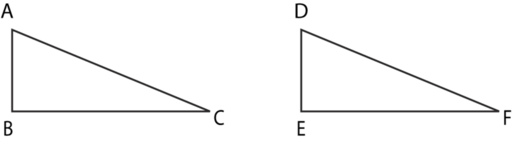
\includegraphics[width=0.45\textwidth]{../images/congruencia02}
    \caption{}
    \label{fig:congruencia01}
\end{figure}
Primero, podemos nombrar los ángulos correspondientes. Los ángulos correspondientes coinciden con ángulos entre los dos triángulos. Los ángulos correspondientes tendrán la misma medida en triángulos congruentes.
\begin{align*}
    \angle A & \cong \angle D \\
    \angle B & \cong \angle E \\
    \angle C & \cong \angle F \\
\end{align*}
Luego, podemos nombrar los lados correspondientes. Los lados correspondientes son lados que coinciden entre los dos triángulos. Tendrán la misma longitud en triángulos congruentes.
\begin{align*}
    \overline{AB} & \cong \overline{DE} \\
    \overline{AC} & \cong \overline{DF} \\
    \overline{BC} & \cong \overline{EF} \\
\end{align*}
%     \begin{tcbraster}[raster columns=2,
%             title=Pregunta \thetcbrasternum,
%             enhanced,colframe=red!50!black,colback=red!10!white]
% \begin{tcolorbox} \include*{../questions/question030a}\end{tcolorbox}
% \begin{tcolorbox} \include*{../questions/question030b}\end{tcolorbox}
% \begin{tcolorbox} \include*{../questions/question030c}\end{tcolorbox}
% \begin{tcolorbox} \include*{../questions/question030d}\end{tcolorbox}
% \begin{tcolorbox} \include*{../questions/question030e}\end{tcolorbox}
% \begin{tcolorbox} \include*{../questions/question030f}\end{tcolorbox}
% \begin{tcolorbox} \include*{../questions/question030g}\end{tcolorbox}
% \begin{tcolorbox} \include*{../questions/question030h}\end{tcolorbox}
% \begin{tcolorbox} \include*{../questions/question030i}\end{tcolorbox}
% \begin{tcolorbox} \include*{../questions/question030j}\end{tcolorbox}
% \begin{tcolorbox} \include*{../questions/question030k}\end{tcolorbox}
% \end{tcbraster}
\begin{questions}
    % \section{Section 1}
    % \vbox{\leftskip\leftmargin Some descriptive text.}
    %\include*{../questions/question030a}
    \include*{../questions/question030b}
    % \include*{../questions/question030c}
    % \include*{../questions/question030d}
    % \include*{../questions/question030e}
    % \include*{../questions/question030f}
    % \include*{../questions/question030g}
    % \include*{../questions/question030h}
    % \include*{../questions/question030i}
    % \include*{../questions/question030j}
    % \include*{../questions/question030k}
\end{questions}

\end{document}